% Inhalte des Papers (grob), Schwerpunkte (Verbesserungen in Tor gegenüber damals existierenden Systemen), Neuerungen in Tor, etc.
%Mal schauen, eher beide...

%-Verbeserungen zu Onion routing:
%aus dem abstract: 
%by adding perfect forward secrecy, 
%congestion control, 
%directory servers,
%integrity checking, 
%configurable exit policies, 
%and a practical design for location-hidden services via rendezvous points.


% How does Tor work? Onion proxy, onion router, TLS link encryption, cells, constructing a circuit, sending data (HTTP, ...)
% Chapter6: Other design decisions: DoS, Exit policies and abuse, dirrectory servers



\section{Tor}

The details mentioned in this section are taken from \cite{tor2004original} if not stated otherwise.

Tor is a circuit-based low-latency service providing anonymous communication improving the concepts of the already explained onion routing. It is designed to anonymize TCP connections. This enables Tor to work with most standard applications of the net like HTTP to visit websites and other application layer protocols.

Users of the network use an \textbf{onion proxy} to connect their TCP connections to the Tor network. They establish a circuit through the network containing several nodes, so-called \textbf{onion routers}. Every onion router just knows his predecessor and successor in the circuit. How this works in detail is covered below. An overview about the exchanged messages can be found in figure  \ref{img_circuit_creation}.

\subsection{Creating circuits}

Tor uses TLS connections between the onion routers to prevent message tampering by external adversaries and providing perfect forward secrecy (see next section). A client who wants to use the network has to establish a circuit consisting of several onion routers incrementally. Let's call the client Alice and the first onion router on her chosen circuit Bob\footnote{
	Traditions have to be preserved!
}. Bob (as well as every other onion router) owns a long-term identity key pair to sign TLS certificates and his router description and a short-term onion key pair used when setting up circuits. .\\ Alice sends Bob a \textit{create} control cell\footnote{
	Tor cells have a fixed size of 512 bytes and always contain circuit identifier, the command and a payload. The command can be \textit{control} for cells which are interpreted by the receiving onion router or \textit{relay} for carrying end-to-end data.
} containing a unused circuit id and a DH\footnote{
	The Diffie-Hellman key exchange is a method to exchange keys over a public network using public-key cryptography. Details can be found in \cite{diffie1976new}.
} key exchange parameter \(g^x\) encrypted with Bob's onion key. Bob decrypts this parameter, computes the shared key \(K = g^{xy}\) and sends Alice a \textit{created} cell containing the circuit identifier and the DH parameter \(g^y\) so that Alice can compute \(K\) too.

\begin{figure}
	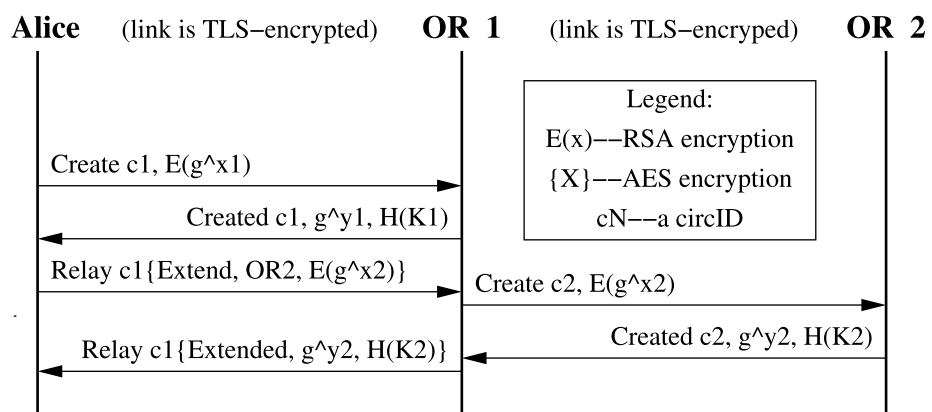
\includegraphics[width=\columnwidth]{img/circuit_creation.png}
	\caption{Creating a circuit with two onion routers. Taken from \cite{tor2004original} and slightly edited.}
	\label{img_circuit_creation}
\end{figure}

When Alice wants to extend this circuit to the next onion router Carol she sends a relay \textit{extend} cell to Bob, which contains the address of Carol as well as a DH parameter \(g^{x_2}\) encrypted with Carols onion key. This data is encrypted symmetrically with AES-128 and the already negotiated key \(K\) between Alice and Bob.\\
Bob decrypts this information, chooses a unused circuit identifier between Carol and him and forwards the information received from Alice to Carol in a new \textit{create} cell. The same process as already described takes place on Carols side and she sends \(g^{y_2}\) back to Bob after computing the key \(K_2 = g^{x_2y_2}\). Bob encrypts this information with \(K\) and sends it back to Alice who can also compute \(K_2\) then. The circuit is extended by another onion router now and Alice has a key shared with Bob and one shared with Carol.

\subsection{Sending TCP data through a circuit}

After having established a circuit Alice can start to send data over the Tor network. This is illustrated below for the simple case of requesting a website. An overview can be found in figure \ref{img_http_request}.

\begin{figure}
	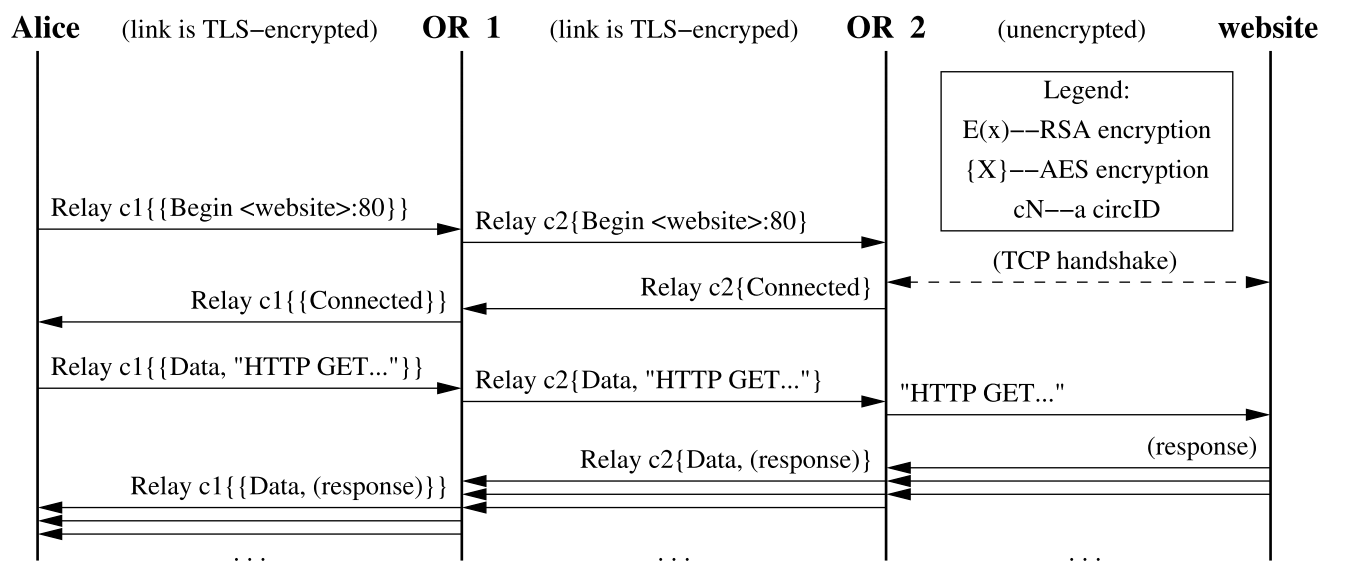
\includegraphics[width=\columnwidth]{img/http_request.png}
	\caption{Requesting the content if a website via HTTP over an established circuit. Taken from \cite{tor2004original} and slightly edited.}
	\label{img_http_request}
\end{figure}

In the first step Alice sends a relay begin cell to open a new TCP stream. The content of the cell (the begin command, a stream identifier, the website address and a digest of the message) is encrypted multiple times with the keys obtained when creating the circuit in order of the onion routers on the circuit. So Alice encrypts the message with Bob's key first and then with Carol's key and sends it to Bob.

Bob decrypts the information the first time and forwards it to Carol. Carol decrypts it the second time, gets the original request from Alice and performs the TCP handshake with the requested webserver. After a successful connection she answers with a \textit{connected} relay cell encrypted with the with Alice negotiated key. Bob encrypts the answer a second time and returns it to Alice who can then decrypt it twice and knows the handshake was successful. Now she can start to send a HTTP request over the established TCP stream packed in relay \textit{data} cells in the same way as before.

But how does Bob know he is not the addressee of the cell during the handshake? This is where the message digest comes into play. Every onion router checks if the message digest he obtains after decrypting a cell is valid for the cell data. If this is the case the cell should be received by him and he can perform the required task (opening a TCP connection in this case). If the message digest is not valid, he forwards the message to the next receiver on the circuit. This topology is called leaky pipe - enabling a user to choose different exit points for streams using just one circuit. 

\subsection{Improvements to onion routing}

While the approaches described in the previous subsection are quite similar to the original onion routing techniques, there are several improvements in Tor which this subsection will cover.

\subsubsection{Directory servers} 
Both - onion routing and Tor - have to give users access to state information about the network (known onion routers and their current states). In the onion routing design the network is flooded with these state informations (similar to normal routing protocols), which can be unreliable, complex and give attackers opportunities to exploit different client knowledge. Tor uses so called \textit{directory servers} to give clients access to the signed current network state. The users get a predefined list of directory servers with their Tor application and contact them periodically via HTTP to update their known network state.

\subsubsection{Rendezvous points and hidden services} 
Previous sections all were dealing with how to prevent traffic analysis through the network to a well-known server. But Tor also has the ability to offer hidden services - servers which real addresses are hidden and which can just be contacted via so-called rendezvous points. This can for example prevent precise DoS-attacks.

An operator can announce several onion routers as contact points for his hidden service and builds circuits to them from his service. A client, who knows about the hidden service, can lookup the contact points and inform a contact point of a chosen onion router where the circuits should connect - the rendezvous point. The connection of both circuits is done by using a rendezvous cookie which is sent to the location point of the hidden service. Once again the Diffie-Hellman key exchange is used to negotiate a shared key between client and server to prevent even the rendezvous point to look into the message content.

The onion routing design used long-living "reply onions", which were used to build a circuit to a hidden server. This approach failed if any onion router on the preestablished path went down or updated his keys.

\subsubsection{Perfect forward secrecy} 
Perfect forward secrecy describes the property of a key exchange protocol. By using ephemeral session keys, which cannot be derived from long-term keys and are deleted when not being required anymore, older messages cannot be decrypted even if the long-term key gets compromised.

The original onion routing suffers from the problem that a single malicious node can record traffic and by compromising following nodes in the circuit making them to decrypt the recorded traffic. 
To avoid this Tor uses an incremental path building design. The initiator negotiates session keys with each node in the circuit. When these keys are deleted after a circuit has been destroyed, the compromised nodes are not able to decrypt the recorded traffic.

Another advantage is the usage of TLS between the onion routers enabling perfect forward secrecy on connection level.

\subsubsection{Congestion control} 
If many users choose the same connection between onion routers in their circuits, it is possible to overload a connection. To avoid this, Tor is able to control the circuit bandwidths in each onion router. It does this by using a TCP like window approach for incoming and outgoing connections.

\subsubsection{Integrity checking} 
Tor uses an end-to-end integrity checksum in its messages, which prevents altering messages in between. Additionally using TLS between the onion routers hampers the altering of data in connections between onion routers.

\subsubsection{Exit policies}
Tor allows onion routers to provide a policy of allowed outgoing connections. This can be used to prohibit or just allow connections to special hosts or to limit the allowed protocols. Because Tor is a volunteer-based network these policies are required to give operators control over routed traffic.

\subsubsection{Leaky-pipe topology}
A final advantage of Tor over onion routing is the already explained leaky pipe topology which allows requests leaving the Tor network in the middle of circuits. This makes traffic analysis even harder for adversaries, because just observing the begin and end of a circuit is not enough anymore.